%%%%%%%%%%%%%%%%%%%%%%%%%%%%%%%%%%%%%%%%%
% University Assignment Title Page 
% LaTeX Template
% Version 1.0 (27/12/12)
%
% This template has been downloaded from:
% http://www.LaTeXTemplates.com
%
% Original author:
% WikiBooks (http://en.wikibooks.org/wiki/LaTeX/Title_Creation)
%
% License:
% CC BY-NC-SA 3.0 (http://creativecommons.org/licenses/by-nc-sa/3.0/)
% 
% Instructions for using this template:
% This title page is capable of being compiled as is. This is not useful for 
% including it in another document. To do this, you have two options: 
%
% 1) Copy/paste everything between \begin{document} and \end{document} 
% starting at \begin{titlepage} and paste this into another LaTeX file where you 
% want your title page.
% OR
% 2) Remove everything outside the \begin{titlepage} and \end{titlepage} and 
% move this file to the same directory as the LaTeX file you wish to add it to. 
% Then add %%%%%%%%%%%%%%%%%%%%%%%%%%%%%%%%%%%%%%%%%
% University Assignment Title Page 
% LaTeX Template
% Version 1.0 (27/12/12)
%
% This template has been downloaded from:
% http://www.LaTeXTemplates.com
%
% Original author:
% WikiBooks (http://en.wikibooks.org/wiki/LaTeX/Title_Creation)
%
% License:
% CC BY-NC-SA 3.0 (http://creativecommons.org/licenses/by-nc-sa/3.0/)
% 
% Instructions for using this template:
% This title page is capable of being compiled as is. This is not useful for 
% including it in another document. To do this, you have two options: 
%
% 1) Copy/paste everything between \begin{document} and \end{document} 
% starting at \begin{titlepage} and paste this into another LaTeX file where you 
% want your title page.
% OR
% 2) Remove everything outside the \begin{titlepage} and \end{titlepage} and 
% move this file to the same directory as the LaTeX file you wish to add it to. 
% Then add %%%%%%%%%%%%%%%%%%%%%%%%%%%%%%%%%%%%%%%%%
% University Assignment Title Page 
% LaTeX Template
% Version 1.0 (27/12/12)
%
% This template has been downloaded from:
% http://www.LaTeXTemplates.com
%
% Original author:
% WikiBooks (http://en.wikibooks.org/wiki/LaTeX/Title_Creation)
%
% License:
% CC BY-NC-SA 3.0 (http://creativecommons.org/licenses/by-nc-sa/3.0/)
% 
% Instructions for using this template:
% This title page is capable of being compiled as is. This is not useful for 
% including it in another document. To do this, you have two options: 
%
% 1) Copy/paste everything between \begin{document} and \end{document} 
% starting at \begin{titlepage} and paste this into another LaTeX file where you 
% want your title page.
% OR
% 2) Remove everything outside the \begin{titlepage} and \end{titlepage} and 
% move this file to the same directory as the LaTeX file you wish to add it to. 
% Then add %%%%%%%%%%%%%%%%%%%%%%%%%%%%%%%%%%%%%%%%%
% University Assignment Title Page 
% LaTeX Template
% Version 1.0 (27/12/12)
%
% This template has been downloaded from:
% http://www.LaTeXTemplates.com
%
% Original author:
% WikiBooks (http://en.wikibooks.org/wiki/LaTeX/Title_Creation)
%
% License:
% CC BY-NC-SA 3.0 (http://creativecommons.org/licenses/by-nc-sa/3.0/)
% 
% Instructions for using this template:
% This title page is capable of being compiled as is. This is not useful for 
% including it in another document. To do this, you have two options: 
%
% 1) Copy/paste everything between \begin{document} and \end{document} 
% starting at \begin{titlepage} and paste this into another LaTeX file where you 
% want your title page.
% OR
% 2) Remove everything outside the \begin{titlepage} and \end{titlepage} and 
% move this file to the same directory as the LaTeX file you wish to add it to. 
% Then add \input{./title_page_1.tex} to your LaTeX file where you want your
% title page.
%
%%%%%%%%%%%%%%%%%%%%%%%%%%%%%%%%%%%%%%%%%

%----------------------------------------------------------------------------------------
%	PACKAGES AND OTHER DOCUMENT CONFIGURATIONS
%----------------------------------------------------------------------------------------

\documentclass[12pt, showidx]{article}

\usepackage[utf8]{inputenc}
\usepackage[T1]{fontenc}
\usepackage{lmodern}
\usepackage{parselines}
\usepackage[portuguese]{babel}
\usepackage{graphicx}
\usepackage{imakeidx}
\usepackage[document]{ragged2e}

\graphicspath{ {images/} }

\makeindex[title = Palavras Chave]

\begin{document}

\begin{titlepage}

\newcommand{\HRule}{\rule{\linewidth}{1mm}} % Defines a new command for the horizontal lines, change thickness here

\center % Center everything on the page
 
%----------------------------------------------------------------------------------------
%	HEADING SECTIONS
%----------------------------------------------------------------------------------------


\includegraphics{feup.jpg}

\textsc{\large Inteligência Artificial}\\[0.5cm] % Major heading such as course name
\textsc{\large 3º ano do Mestrado Integrado em Engenharia Informática e Computação}\\[0.5cm] % Minor heading such as course title

%----------------------------------------------------------------------------------------
%	TITLE SECTION
%----------------------------------------------------------------------------------------

\HRule \\[0.4cm]
{ \huge \bfseries Otimização da gestão de projetos}\\[0.2cm] % Title of your document
\HRule \\[1cm]
 
%----------------------------------------------------------------------------------------
%	AUTHOR SECTION
%----------------------------------------------------------------------------------------


% If you don't want a supervisor, uncomment the two lines below and remove the section above
\Large \emph{Authors:}\\
Duarte \textsc{Pinto}\\[0cm] - up201304777 
- up201304777@fe.up.pt\\[0cm]
Filipa \textsc{Ramos}\\[0cm] - up201305378
- up201305378@fe.up.pt\\[0cm] 
Gustavo \textsc{Silva}\\[0cm] - up201304143
- up201304143@fe.up.pt\\[1cm] % Your name

%----------------------------------------------------------------------------------------
%	DATE SECTION
%----------------------------------------------------------------------------------------

{\large \today}\\[0cm] % Date, change the \today to a set date if you want to be precise

%----------------------------------------------------------------------------------------
%	TABLE OF CONTENTS & LISTS OF FIGURES AND TABLES
%----------------------------------------------------------------------------------------

\tableofcontents

%----------------------------------------------------------------------------------------
%	INTRODUÇÃO
%----------------------------------------------------------------------------------------

\section{Introdução} 

\justify\normalsize
No âmbito da unidade curricular de Inteligência Artificial pretende-se desenvolver um programa que, com base em algoritmos genéticos e arrefecimento simulado, faça a gestão de um projeto balançando os elementos participantes e as tarefas a realizar do mesmo. O sistema é composto por um conjunto de tarefas que pertencem ao projeto em análise. Cada tarefa tem uma competência indispensável ao seu cumprimento e uma duração. Cada elemento tem um conjunto de competências sendo que o mesmo tem um nível de capacidade para cumprir cada uma. A gestão a ser realizada tem em vista minimizar o tempo ocupado para satisfazer todas as tarefas do projeto usando a melhor combinação de elementos para cada tarefa. Será feita uma análise comparativa entre o desempenho das solução encontradas com algoritmos genéticos e arrefecimento simulado. 

Os objetivos principais do projeto passam pela exploração da implementação prática dos algoritmos genéticos e do algoritmo de arrefecimento simulado. Através dos dados obtidos, visa-se também realizar uma comparação da solução encontrada com ambos os algoritmos. Este processo irá fomentar o conhecimento adquirido, evidenciando as vantagens principais de cada algoritmo e as suas dicotomias principais.  

Espera-se que surjam dificuldades na implementação prática dos algoritmos estudados teoricamente, principalmente na construção dos cromossomas pois existem dúvidas em relação à sua influência na eficiência da solução encontrada. Para além disto, a melhor adaptação da função de avaliação ao problema por forma a obter os melhores resultados revela-se um processo tumultuoso. Os membros decidiram optar por otimizar o tempo utilizado a concluir todas as tarefas do projeto em estudo. Desta forma, a melhor solução será a que implicará um menor tempo de conclusão do projeto em questão.

%----------------------------------------------------------------------------------------

\newpage % Start the article content on the second page, remove this if you have a longer abstract that goes onto the second page

%----------------------------------------------------------------------------------------
%	ESPECIFICAÇÃO
%----------------------------------------------------------------------------------------

\section{Especificação}

\subsection{Problematização}
\justify\normalsize
O sistema tem por objetivo otimizar a atribuição de membros por tarefas num dado projeto. Os dados do mesmo são introduzidos por input através de um ficheiro.

Um projeto em análise caracteriza-se por um conjunto de tarefas (\index{Task} Task) a cumprir, tendo estas um nome (por motivos de identificação) e uma duração. Existe ainda um conjunto de elementos (\index{Element} Element) que podem ser atribuídos a essas mesmas tarefas. Um elemento é identificado por um nome e tem uma lista de competências (\index{Skill} Skill) avaliadas em função da sua capacidade. Por exemplo, o elemento "joão" tem competências na área da informática a um nível 6 e na área da economia com nível 10.

\subsection{Aquitetura}
\justify\normalsize
O projeto foi dividido em três "packages" principais que representam os três níveis mais importantes. Um dos packages diz respeito às classes que guardam informação sobre as tarefas, os elementos e as competências. Os outros dois dizem respeito à implementação do algoritmo genético ou do arrefecimento simulado.

A arquitetura pensada para o projeto passa pela implementação de três classes principais que interagem entre si próprias. A classe "Task" representa uma tarefa e guarda a sua duração. Um elemento é representado pela classe "Element" que mantém a identificação do mesmo. A classe "Skill" corresponde a uma competência. Estas ligam-se entre si por forma a que um elemento tenha vários skills e um skill tenha várias tarefas tal como é visível na figura \ref{fig:uml}.

\begin{figure}[h]
  \centering
    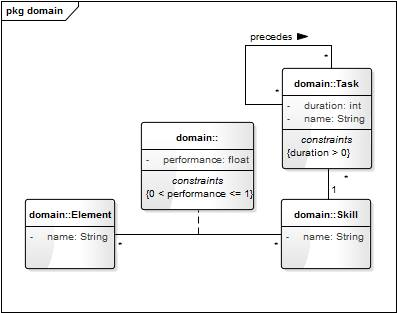
\includegraphics[width=10cm, height = 10cm]{uml.jpg}
  \caption{Diagrama de classes UML}
  \label{fig:uml}
\end{figure}

\subsection{Fases}
\justify\normalsize 
O projeto será dividido em fases de trabalho. A inicial passa pelo desenvolvimento da arquitetura explicitada em cima. Seguidamente, proceder-se-á implementação dos \index{Algortimos Genéticos} algoritmos genéticos. Finalmente, será desenvolvido o arrefecimento simulado. As fases abordadas até ao presente relatório foram as duas primeiras. A arquitetura explicitada pelo diagrama de classes uml já foi implementada e a obtenção de solução por algoritmos genéticos encontra-se numa fase avançada.

\subsection{Algoritmos Genéticos}
\justify\normalsize
Explicar o algoritmo usado:
	- estrutura do cromossoma
	- função de avaliação
	- seleção
	- cruzamento
	- mutações

\subsection{Arrefecimento Simulado}
\justify\normalsize
Explicar o algoritmo usado.

\section{Trabalho Realizado}
\justify\normalsize
Incluir trechos do código já implementado.

\section{Testes}
\justify\normalsize
Explicar os testes planeados.

\section{Conclusões}
\justify\normalsize
Conclusões retiradas.

\printindex

\end{titlepage}
\end{document} to your LaTeX file where you want your
% title page.
%
%%%%%%%%%%%%%%%%%%%%%%%%%%%%%%%%%%%%%%%%%

%----------------------------------------------------------------------------------------
%	PACKAGES AND OTHER DOCUMENT CONFIGURATIONS
%----------------------------------------------------------------------------------------

\documentclass[12pt, showidx]{article}

\usepackage[utf8]{inputenc}
\usepackage[T1]{fontenc}
\usepackage{lmodern}
\usepackage{parselines}
\usepackage[portuguese]{babel}
\usepackage{graphicx}
\usepackage{imakeidx}
\usepackage[document]{ragged2e}

\graphicspath{ {images/} }

\makeindex[title = Palavras Chave]

\begin{document}

\begin{titlepage}

\newcommand{\HRule}{\rule{\linewidth}{1mm}} % Defines a new command for the horizontal lines, change thickness here

\center % Center everything on the page
 
%----------------------------------------------------------------------------------------
%	HEADING SECTIONS
%----------------------------------------------------------------------------------------


\includegraphics{feup.jpg}

\textsc{\large Inteligência Artificial}\\[0.5cm] % Major heading such as course name
\textsc{\large 3º ano do Mestrado Integrado em Engenharia Informática e Computação}\\[0.5cm] % Minor heading such as course title

%----------------------------------------------------------------------------------------
%	TITLE SECTION
%----------------------------------------------------------------------------------------

\HRule \\[0.4cm]
{ \huge \bfseries Otimização da gestão de projetos}\\[0.2cm] % Title of your document
\HRule \\[1cm]
 
%----------------------------------------------------------------------------------------
%	AUTHOR SECTION
%----------------------------------------------------------------------------------------


% If you don't want a supervisor, uncomment the two lines below and remove the section above
\Large \emph{Authors:}\\
Duarte \textsc{Pinto}\\[0cm] - up201304777 
- up201304777@fe.up.pt\\[0cm]
Filipa \textsc{Ramos}\\[0cm] - up201305378
- up201305378@fe.up.pt\\[0cm] 
Gustavo \textsc{Silva}\\[0cm] - up201304143
- up201304143@fe.up.pt\\[1cm] % Your name

%----------------------------------------------------------------------------------------
%	DATE SECTION
%----------------------------------------------------------------------------------------

{\large \today}\\[0cm] % Date, change the \today to a set date if you want to be precise

%----------------------------------------------------------------------------------------
%	TABLE OF CONTENTS & LISTS OF FIGURES AND TABLES
%----------------------------------------------------------------------------------------

\tableofcontents

%----------------------------------------------------------------------------------------
%	INTRODUÇÃO
%----------------------------------------------------------------------------------------

\section{Introdução} 

\justify\normalsize
No âmbito da unidade curricular de Inteligência Artificial pretende-se desenvolver um programa que, com base em algoritmos genéticos e arrefecimento simulado, faça a gestão de um projeto balançando os elementos participantes e as tarefas a realizar do mesmo. O sistema é composto por um conjunto de tarefas que pertencem ao projeto em análise. Cada tarefa tem uma competência indispensável ao seu cumprimento e uma duração. Cada elemento tem um conjunto de competências sendo que o mesmo tem um nível de capacidade para cumprir cada uma. A gestão a ser realizada tem em vista minimizar o tempo ocupado para satisfazer todas as tarefas do projeto usando a melhor combinação de elementos para cada tarefa. Será feita uma análise comparativa entre o desempenho das solução encontradas com algoritmos genéticos e arrefecimento simulado. 

Os objetivos principais do projeto passam pela exploração da implementação prática dos algoritmos genéticos e do algoritmo de arrefecimento simulado. Através dos dados obtidos, visa-se também realizar uma comparação da solução encontrada com ambos os algoritmos. Este processo irá fomentar o conhecimento adquirido, evidenciando as vantagens principais de cada algoritmo e as suas dicotomias principais.  

Espera-se que surjam dificuldades na implementação prática dos algoritmos estudados teoricamente, principalmente na construção dos cromossomas pois existem dúvidas em relação à sua influência na eficiência da solução encontrada. Para além disto, a melhor adaptação da função de avaliação ao problema por forma a obter os melhores resultados revela-se um processo tumultuoso. Os membros decidiram optar por otimizar o tempo utilizado a concluir todas as tarefas do projeto em estudo. Desta forma, a melhor solução será a que implicará um menor tempo de conclusão do projeto em questão.

%----------------------------------------------------------------------------------------

\newpage % Start the article content on the second page, remove this if you have a longer abstract that goes onto the second page

%----------------------------------------------------------------------------------------
%	ESPECIFICAÇÃO
%----------------------------------------------------------------------------------------

\section{Especificação}

\subsection{Problematização}
\justify\normalsize
O sistema tem por objetivo otimizar a atribuição de membros por tarefas num dado projeto. Os dados do mesmo são introduzidos por input através de um ficheiro.

Um projeto em análise caracteriza-se por um conjunto de tarefas (\index{Task} Task) a cumprir, tendo estas um nome (por motivos de identificação) e uma duração. Existe ainda um conjunto de elementos (\index{Element} Element) que podem ser atribuídos a essas mesmas tarefas. Um elemento é identificado por um nome e tem uma lista de competências (\index{Skill} Skill) avaliadas em função da sua capacidade. Por exemplo, o elemento "joão" tem competências na área da informática a um nível 6 e na área da economia com nível 10.

\subsection{Aquitetura}
\justify\normalsize
O projeto foi dividido em três "packages" principais que representam os três níveis mais importantes. Um dos packages diz respeito às classes que guardam informação sobre as tarefas, os elementos e as competências. Os outros dois dizem respeito à implementação do algoritmo genético ou do arrefecimento simulado.

A arquitetura pensada para o projeto passa pela implementação de três classes principais que interagem entre si próprias. A classe "Task" representa uma tarefa e guarda a sua duração. Um elemento é representado pela classe "Element" que mantém a identificação do mesmo. A classe "Skill" corresponde a uma competência. Estas ligam-se entre si por forma a que um elemento tenha vários skills e um skill tenha várias tarefas tal como é visível na figura \ref{fig:uml}.

\begin{figure}[h]
  \centering
    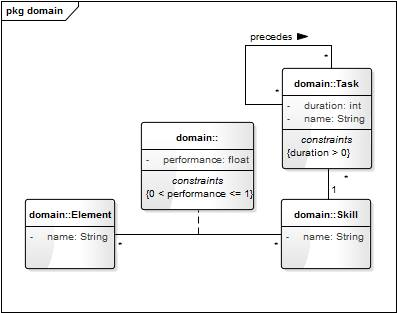
\includegraphics[width=10cm, height = 10cm]{uml.jpg}
  \caption{Diagrama de classes UML}
  \label{fig:uml}
\end{figure}

\subsection{Fases}
\justify\normalsize 
O projeto será dividido em fases de trabalho. A inicial passa pelo desenvolvimento da arquitetura explicitada em cima. Seguidamente, proceder-se-á implementação dos \index{Algortimos Genéticos} algoritmos genéticos. Finalmente, será desenvolvido o arrefecimento simulado. As fases abordadas até ao presente relatório foram as duas primeiras. A arquitetura explicitada pelo diagrama de classes uml já foi implementada e a obtenção de solução por algoritmos genéticos encontra-se numa fase avançada.

\subsection{Algoritmos Genéticos}
\justify\normalsize
Explicar o algoritmo usado:
	- estrutura do cromossoma
	- função de avaliação
	- seleção
	- cruzamento
	- mutações

\subsection{Arrefecimento Simulado}
\justify\normalsize
Explicar o algoritmo usado.

\section{Trabalho Realizado}
\justify\normalsize
Incluir trechos do código já implementado.

\section{Testes}
\justify\normalsize
Explicar os testes planeados.

\section{Conclusões}
\justify\normalsize
Conclusões retiradas.

\printindex

\end{titlepage}
\end{document} to your LaTeX file where you want your
% title page.
%
%%%%%%%%%%%%%%%%%%%%%%%%%%%%%%%%%%%%%%%%%

%----------------------------------------------------------------------------------------
%	PACKAGES AND OTHER DOCUMENT CONFIGURATIONS
%----------------------------------------------------------------------------------------

\documentclass[12pt, showidx]{article}

\usepackage[utf8]{inputenc}
\usepackage[T1]{fontenc}
\usepackage{lmodern}
\usepackage{parselines}
\usepackage[portuguese]{babel}
\usepackage{graphicx}
\usepackage{imakeidx}
\usepackage[document]{ragged2e}

\graphicspath{ {images/} }

\makeindex[title = Palavras Chave]

\begin{document}

\begin{titlepage}

\newcommand{\HRule}{\rule{\linewidth}{1mm}} % Defines a new command for the horizontal lines, change thickness here

\center % Center everything on the page
 
%----------------------------------------------------------------------------------------
%	HEADING SECTIONS
%----------------------------------------------------------------------------------------


\includegraphics{feup.jpg}

\textsc{\large Inteligência Artificial}\\[0.5cm] % Major heading such as course name
\textsc{\large 3º ano do Mestrado Integrado em Engenharia Informática e Computação}\\[0.5cm] % Minor heading such as course title

%----------------------------------------------------------------------------------------
%	TITLE SECTION
%----------------------------------------------------------------------------------------

\HRule \\[0.4cm]
{ \huge \bfseries Otimização da gestão de projetos}\\[0.2cm] % Title of your document
\HRule \\[1cm]
 
%----------------------------------------------------------------------------------------
%	AUTHOR SECTION
%----------------------------------------------------------------------------------------


% If you don't want a supervisor, uncomment the two lines below and remove the section above
\Large \emph{Authors:}\\
Duarte \textsc{Pinto}\\[0cm] - up201304777 
- up201304777@fe.up.pt\\[0cm]
Filipa \textsc{Ramos}\\[0cm] - up201305378
- up201305378@fe.up.pt\\[0cm] 
Gustavo \textsc{Silva}\\[0cm] - up201304143
- up201304143@fe.up.pt\\[1cm] % Your name

%----------------------------------------------------------------------------------------
%	DATE SECTION
%----------------------------------------------------------------------------------------

{\large \today}\\[0cm] % Date, change the \today to a set date if you want to be precise

%----------------------------------------------------------------------------------------
%	TABLE OF CONTENTS & LISTS OF FIGURES AND TABLES
%----------------------------------------------------------------------------------------

\tableofcontents

%----------------------------------------------------------------------------------------
%	INTRODUÇÃO
%----------------------------------------------------------------------------------------

\section{Introdução} 

\justify\normalsize
No âmbito da unidade curricular de Inteligência Artificial pretende-se desenvolver um programa que, com base em algoritmos genéticos e arrefecimento simulado, faça a gestão de um projeto balançando os elementos participantes e as tarefas a realizar do mesmo. O sistema é composto por um conjunto de tarefas que pertencem ao projeto em análise. Cada tarefa tem uma competência indispensável ao seu cumprimento e uma duração. Cada elemento tem um conjunto de competências sendo que o mesmo tem um nível de capacidade para cumprir cada uma. A gestão a ser realizada tem em vista minimizar o tempo ocupado para satisfazer todas as tarefas do projeto usando a melhor combinação de elementos para cada tarefa. Será feita uma análise comparativa entre o desempenho das solução encontradas com algoritmos genéticos e arrefecimento simulado. 

Os objetivos principais do projeto passam pela exploração da implementação prática dos algoritmos genéticos e do algoritmo de arrefecimento simulado. Através dos dados obtidos, visa-se também realizar uma comparação da solução encontrada com ambos os algoritmos. Este processo irá fomentar o conhecimento adquirido, evidenciando as vantagens principais de cada algoritmo e as suas dicotomias principais.  

Espera-se que surjam dificuldades na implementação prática dos algoritmos estudados teoricamente, principalmente na construção dos cromossomas pois existem dúvidas em relação à sua influência na eficiência da solução encontrada. Para além disto, a melhor adaptação da função de avaliação ao problema por forma a obter os melhores resultados revela-se um processo tumultuoso. Os membros decidiram optar por otimizar o tempo utilizado a concluir todas as tarefas do projeto em estudo. Desta forma, a melhor solução será a que implicará um menor tempo de conclusão do projeto em questão.

%----------------------------------------------------------------------------------------

\newpage % Start the article content on the second page, remove this if you have a longer abstract that goes onto the second page

%----------------------------------------------------------------------------------------
%	ESPECIFICAÇÃO
%----------------------------------------------------------------------------------------

\section{Especificação}

\subsection{Problematização}
\justify\normalsize
O sistema tem por objetivo otimizar a atribuição de membros por tarefas num dado projeto. Os dados do mesmo são introduzidos por input através de um ficheiro.

Um projeto em análise caracteriza-se por um conjunto de tarefas (\index{Task} Task) a cumprir, tendo estas um nome (por motivos de identificação) e uma duração. Existe ainda um conjunto de elementos (\index{Element} Element) que podem ser atribuídos a essas mesmas tarefas. Um elemento é identificado por um nome e tem uma lista de competências (\index{Skill} Skill) avaliadas em função da sua capacidade. Por exemplo, o elemento "joão" tem competências na área da informática a um nível 6 e na área da economia com nível 10.

\subsection{Aquitetura}
\justify\normalsize
O projeto foi dividido em três "packages" principais que representam os três níveis mais importantes. Um dos packages diz respeito às classes que guardam informação sobre as tarefas, os elementos e as competências. Os outros dois dizem respeito à implementação do algoritmo genético ou do arrefecimento simulado.

A arquitetura pensada para o projeto passa pela implementação de três classes principais que interagem entre si próprias. A classe "Task" representa uma tarefa e guarda a sua duração. Um elemento é representado pela classe "Element" que mantém a identificação do mesmo. A classe "Skill" corresponde a uma competência. Estas ligam-se entre si por forma a que um elemento tenha vários skills e um skill tenha várias tarefas tal como é visível na figura \ref{fig:uml}.

\begin{figure}[h]
  \centering
    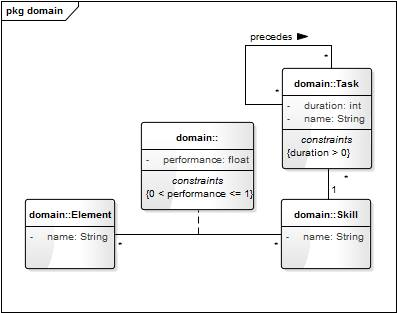
\includegraphics[width=10cm, height = 10cm]{uml.jpg}
  \caption{Diagrama de classes UML}
  \label{fig:uml}
\end{figure}

\subsection{Fases}
\justify\normalsize 
O projeto será dividido em fases de trabalho. A inicial passa pelo desenvolvimento da arquitetura explicitada em cima. Seguidamente, proceder-se-á implementação dos \index{Algortimos Genéticos} algoritmos genéticos. Finalmente, será desenvolvido o arrefecimento simulado. As fases abordadas até ao presente relatório foram as duas primeiras. A arquitetura explicitada pelo diagrama de classes uml já foi implementada e a obtenção de solução por algoritmos genéticos encontra-se numa fase avançada.

\subsection{Algoritmos Genéticos}
\justify\normalsize
Explicar o algoritmo usado:
	- estrutura do cromossoma
	- função de avaliação
	- seleção
	- cruzamento
	- mutações

\subsection{Arrefecimento Simulado}
\justify\normalsize
Explicar o algoritmo usado.

\section{Trabalho Realizado}
\justify\normalsize
Incluir trechos do código já implementado.

\section{Testes}
\justify\normalsize
Explicar os testes planeados.

\section{Conclusões}
\justify\normalsize
Conclusões retiradas.

\printindex

\end{titlepage}
\end{document} to your LaTeX file where you want your
% title page.
%
%%%%%%%%%%%%%%%%%%%%%%%%%%%%%%%%%%%%%%%%%

%----------------------------------------------------------------------------------------
%	PACKAGES AND OTHER DOCUMENT CONFIGURATIONS
%----------------------------------------------------------------------------------------

\documentclass[12pt]{article}

\usepackage[utf8]{inputenc}
\usepackage[T1]{fontenc}
\usepackage{lmodern}
\usepackage{parselines}
\usepackage[portuguese]{babel}
\usepackage{graphicx}
\usepackage[document]{ragged2e}
\usepackage{listings}
\usepackage{xcolor}
\usepackage[margin=0.8in]{geometry}		
\usepackage{amsmath}
\usepackage{hyperref}
\usepackage{url}

\graphicspath{ {images/} }

\colorlet{punct}{red!60!black}
\definecolor{background}{HTML}{EEEEEE}
\definecolor{delim}{RGB}{20,105,176}
\colorlet{numb}{magenta!60!black}


\lstdefinelanguage{json}{
    basicstyle=\normalfont\ttfamily,
    numbers=left,
    numberstyle=\scriptsize,
    stepnumber=1,
    numbersep=8pt,
    showstringspaces=false,
    breaklines=true,
    frame=lines,
    backgroundcolor=\color{background},
    literate=
     *{0}{{{\color{numb}0}}}{1}
      {1}{{{\color{numb}1}}}{1}
      {2}{{{\color{numb}2}}}{1}
      {3}{{{\color{numb}3}}}{1}
      {4}{{{\color{numb}4}}}{1}
      {5}{{{\color{numb}5}}}{1}
      {6}{{{\color{numb}6}}}{1}
      {7}{{{\color{numb}7}}}{1}
      {8}{{{\color{numb}8}}}{1}
      {9}{{{\color{numb}9}}}{1}
      {:}{{{\color{punct}{:}}}}{1}
      {,}{{{\color{punct}{,}}}}{1}
      {\{}{{{\color{delim}{\{}}}}{1}
      {\}}{{{\color{delim}{\}}}}}{1}
      {[}{{{\color{delim}{[}}}}{1}
      {]}{{{\color{delim}{]}}}}{1},
}

\definecolor{dkgreen}{rgb}{0,0.6,0}
\definecolor{gray}{rgb}{0.5,0.5,0.5}
\definecolor{mauve}{rgb}{0.58,0,0.82}

\lstset{frame=tb,
  language=Java,
  aboveskip=3mm,
  belowskip=3mm,
  showstringspaces=false,
  columns=flexible,
  basicstyle={\small\ttfamily},
  numbers=none,
  numberstyle=\tiny\color{gray},
  keywordstyle=\color{blue},
  commentstyle=\color{dkgreen},
  stringstyle=\color{mauve},
  breaklines=true,
  breakatwhitespace=true,
  tabsize=3
}

\begin{document}

\begin{titlepage}

\newcommand{\HRule}{\rule{\linewidth}{1mm}} % Defines a new command for the horizontal lines, change thickness here

\center % Center everything on the page
 
%----------------------------------------------------------------------------------------
%	HEADING SECTIONS
%----------------------------------------------------------------------------------------


\includegraphics{feup.jpg}

\textsc{\large Inteligência Artificial}\\[0.8cm] % Major heading such as course name
\textsc{\large 3º ano do Mestrado Integrado em Engenharia Informática e Computação}\\[0.8cm] % Minor heading such as course title

%----------------------------------------------------------------------------------------
%	TITLE SECTION
%----------------------------------------------------------------------------------------

\HRule \\[1.2cm]
{ \huge \bfseries Otimização da gestão de projetos}\\[0.6cm] % Title of your document
\HRule \\[3cm]
 
%----------------------------------------------------------------------------------------
%	AUTHOR SECTION
%----------------------------------------------------------------------------------------


% If you don't want a supervisor, uncomment the two lines below and remove the section above
\Large \emph{Authors:}\\[0.5cm] \normalsize
Duarte \textsc{Pinto}\\[0.1cm] - up201304777 
- up201304777@fe.up.pt\\[0.1cm]
Filipa \textsc{Ramos}\\[0.1cm] - up201305378
- up201305378@fe.up.pt\\[0.1cm] 
Gustavo \textsc{Silva}\\[0.1cm] - up201304143
- up201304143@fe.up.pt\\[3cm] % Your name

%----------------------------------------------------------------------------------------
%	DATE SECTION
%----------------------------------------------------------------------------------------

{\large \today}\\[0cm] % Date, change the \today to a set date if you want to be precise

%----------------------------------------------------------------------------------------
%	TABLE OF CONTENTS & LISTS OF FIGURES AND TABLES
%----------------------------------------------------------------------------------------

\tableofcontents

%----------------------------------------------------------------------------------------
%	INTRODUÇÃO
%----------------------------------------------------------------------------------------

\section{Introdução} 

\justify\normalsize
No âmbito da unidade curricular de Inteligência Artificial pretende-se desenvolver um programa que, com base em algoritmos genéticos e arrefecimento simulado, faça a gestão de um projeto balançando os elementos participantes e as tarefas a realizar do mesmo. O sistema é composto por um conjunto de tarefas que pertencem ao projeto em análise e um conjunto de elementos que as podem realizar. A gestão a ser realizada tem em vista minimizar o tempo ocupado para satisfazer todas as tarefas do projeto usando a melhor combinação de elementos para cada tarefa. Será feita uma análise comparativa entre o desempenho das solução encontradas com algoritmos genéticos e arrefecimento simulado. 

Os objetivos principais do projeto passam pela exploração da implementação prática dos algoritmos genéticos e do algoritmo de arrefecimento simulado. O processo de análise comparativa irá fomentar o conhecimento adquirido, evidenciando as vantagens principais de cada algoritmo e as suas dicotomias fundamentais.  

Espera-se que surjam dificuldades na implementação prática dos algoritmos estudados teoricamente, principalmente na construção dos cromossomas pois existem dúvidas em relação à sua influência na eficiência da solução encontrada. Para além disto, a melhor adaptação da função de avaliação ao problema por forma a obter os melhores resultados revela-se um processo tumultuoso. Os membros decidiram optar por otimizar o tempo utilizado a concluir todas as tarefas do projeto em estudo. Desta forma, a melhor solução será a que implicará um menor tempo de conclusão do projeto em questão.

%----------------------------------------------------------------------------------------

\newpage % Start the article content on the second page, remove this if you have a longer abstract that goes onto the second page

%----------------------------------------------------------------------------------------
%	ESPECIFICAÇÃO
%----------------------------------------------------------------------------------------

\section{Especificação}

\subsection{Problematização}
\justify\normalsize
O sistema tem por objetivo otimizar a atribuição de membros por tarefas num dado projeto. Os dados do mesmo são introduzidos por input através de um ficheiro.

Um projeto em análise caracteriza-se por um conjunto de tarefas (Task) a cumprir, tendo estas um nome (plor motivos de identificação) e uma duração. Existe ainda um conjunto de elementos (Element) que podem ser atribuídos a essas mesmas tarefas. Um elemento é identificado por um nome e tem uma lista de competências (Skill) avaliadas em função da sua capacidade. Por exemplo, o elemento "joão" tem competências na área da informática a um nível 6 e na área da economia com nível 10.

\subsection{Aquitetura}
\justify\normalsize
O projeto foi dividido em três "packages" principais que representam os três níveis mais importantes. Um dos packages diz respeito às classes que guardam informação sobre as tarefas, os elementos e as competências. Os outros dois dizem respeito à implementação do algoritmo genético ou do arrefecimento simulado.

A arquitetura pensada para o projeto passa pela implementação de três classes principais que interagem entre si próprias. A classe "Task" representa uma tarefa e guarda a sua duração. Um elemento é representado pela classe "Element" que mantém a identificação do mesmo. A classe "Skill" corresponde a uma competência. Estas ligam-se entre si por forma a que um elemento tenha vários skills e um skill tenha várias tarefas tal como é visível na figura \ref{uml}. A relação que se pretende obter será a que liga os elementos a tarefas.

\begin{figure}[h!]
  \centering
    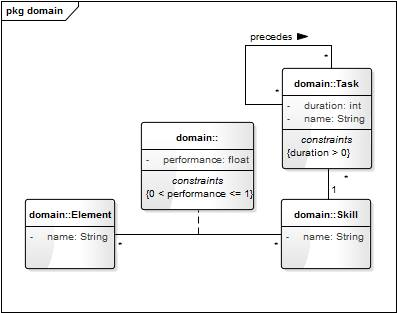
\includegraphics[width=10.5cm, height = 9cm]{uml.jpg}
  \caption{Diagrama de classes UML}
  \label{uml}
\end{figure}

\newpage

\subsection{Formato do input}

O input será colhido de um ficheiro de formato \textit{json} e será estrutrurado conforme está representado no exemplo apresentado a seguir. 

\begin{lstlisting}[language=json,firstnumber=1]
{ 
  "skills": 
      [ "Z", "Y" ], 
   "tasks": [
     { "name": "A", "skill": 0},
     { "name": "B",  "skill": 1}],
   "elements": [
      { "name": "Duarte Pinto", "skills": [ [0, 0.5], [2, 0.1] ]},
      { "name": "Filipa Ramos", "skills": [ [0,1.0]]},
      { "name": "Gustavo Silva", "skills": [ [1, 0.5],  [2, 0.1] ]}]
}
\end{lstlisting}

\subsection{Fases}
\justify\normalsize 
O projeto será dividido em fases de trabalho. A inicial passa pelo desenvolvimento da arquitetura supracitada. Seguidamente, proceder-se-á implementação dos algoritmos genéticos. Finalmente, será desenvolvido o arrefecimento simulado. Após terem sido terminados ambos os algoritmos será realizada a análise comparativa entre os dois, sendo esta a fase final do projeto.

%----------------------------------------------------------------------------------------
%	ALGORITMOS GENÉTICOS
%----------------------------------------------------------------------------------------

\subsection{Algoritmos Genéticos}

\subsubsection{Estrutura do Cromossoma}
\justify\normalsize
A construção dos cromossomas segue a ordem das precedências de tarefas. Assim, o mesmo é composto pelo id da tarefa seguido de 0 ou 1 para cada elemento, sendo que 1 significa que o membro trabalhou na tarefa e 0 significa que o elemento não trabalhou na tarefa. Desta forma, o cromossoma final será composto por x blocos, sendo que x é o número de tarefas existentes. Cada bloco terá tamanho variável dependente do projeto em análise - conforme o número de elementos total e o número de bits necessários para representar a tarefa com um identificador. A fórmula utilizada para cálculo do número de bits máximo do identificador é a apresentada na equação \ref{equação 1}.

\begin{figure}[!ht]
\begin{equation} \label{equação 1}
\lfloor (\dfrac{\log_{10}(size-1)}{log_{10}(2)+1} \rfloor
\end{equation}
\caption{Fórmula para calcular o número de bits máximo para representar com um id binário todas as tarefas (size equivale ao número de tarefas).}
\end{figure}

Por exemplo, se o projeto em análise tiver duas tarefas e dois membros um dos cromossomas da população poderá ser o representado na figura \ref{cromossoma}. Neste caso teríamos os membros 1 e 3 alocados na primeira tarefa e, na segunda, apenas o membro 2. A tarefa com id 0 teria precedência à tarefa com id 1 ou seriam concorrentes.

\begin{figure}[h!]
  \centering
    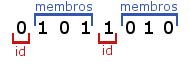
\includegraphics[width=6cm, height = 1.8cm]{cromossoma.png}
  \caption{Cromossoma exemplificativo}
  \label{cromossoma}
\end{figure}

\subsubsection{Função de Avaliação}

A função de avaliação implementada procura avaliar os cromossomas da população tendo por base o tempo total de compleção das tarefas todas do projeto. Assim, um cromossoma com menor valor de \textit{fitness} será mais apto visto que terminou as tarefas em menor tempo. Esta função trata variadas situações extraordinárias. No caso de haverem duas tarefas sem precedências entre si, é procurada a primeira tarefa que possa ser executada. Para além disto, se houverem tarefas sem qualquer precedência, estas serão tratadas depois das que implicam precedências.

\subsubsection{Seleção}

A seleção é feita por uma roleta aleatória que gera valores como está representado no excerto de código a seguir. Estes valores implicam um valor aleatório multiplicado pelo \textit{fitness} total da população. A este valor é subtraído o do \textit{fitness} individual de cada cromossoma. Os selecionados são os que têm menor valor final.  A seleção elitista pode implicar um cromossoma ou mais, sendo este valor escolhido conforme o que se pretende testar.

\begin{lstlisting}[frame=single, language=java,numbers=left,numberfirstline=true]  
for (int i = 0; i < amountToSelect; i++) {
	double d = random.nextDouble() * population.getTotalFitness();	
	for(int j = 0; j < population.getSize(); j++) {		
		d -= population.getChromosome(j).getFitness();		
		if (d <= 0){
			selected[i] = population.getChromosome(j);
			break;}
	}
}
\end{lstlisting}

\subsubsection{Cruzamento}

O cruzamento será aplicado de três maneiras distintas, sendo feita uma análise da eficiência de cada um dos métodos por forma a obter o mais eficaz. Assim, espera-se testar os seguintes tipos de cruzamentos:

\begin{enumerate}
	\item Cruzamento entre tarefas
		\begin{description}
			\item Troca de tarefas entre cromossomas incluindo o id e os elementos.
		\end{description}
	\item Cruzamento dos elementos entre tarefas
		\begin{description}
			\item Troca dos elementos de uma tarefa com os elementos de outra tarefa noutro cromossoma.
		\end{description}
	\item Cruzamento de elementos da mesma tarefa
		\begin{description}
			\item Troca de elementos de uma tarefa com os elementos da mesma tarefa de outro cromossoma.
		\end{description}
\end{enumerate}

\subsubsection{Mutações}

A mutação ocorre a uma taxa variável, sendo esta selecionada conforme os testes pretendidos. A mutação exclui os cromossomas elitistas, tendo por base o princípio de que um cromossoma elitista tem a melhor seleção de genes e, após uma mutação, essa combinação pode ser alterada para uma pior. São gerados valores aleatórios para cada cromossoma numa roleta e, se este for menor que o valor da taxa de mutação, é trocado o bit que resulta do resto da divisão da posição do mesmo no cromossoma pelo comprimento total do cromossoma.

%----------------------------------------------------------------------------------------
%	ARREFECIMENTO SIMULADO
%----------------------------------------------------------------------------------------

\subsection{Arrefecimento Simulado}
\justify\normalsize

Quando adaptado de maneira eficiente o algorítmo de Arrefecimento Simulado é característico pela facilidade de implementação e pela rapidez de convergência do resultado.

Para este projecto optamos por representar a nossa solução através de uma lista de tasks.

\subsubsection{Representação}
A representação da solução é importante pois tem que permitir a geração rápida do próximo estado e rápido calculo do 	$\Delta$E.

Para tal colocamos as tarefas numa lista ordenada de tasks onde cada task aparece numa posição depois de todos os seus antecessores e antes dos seus sucessores e onde as tasks mais pequenas têm prioridade(aparecem primeiro na lista) sobre as tasks mais pesadas.

\subsubsection{Atribuição dos tempos iniciais}
Para atribuir os tempos iniciais de cada tarefa executamos um ciclo onde cada iteração representa a passagem de um \textit{sprint}, de duração é varíavel. Começamos com \textit{i} = 0, percorremos a lista e tentamos atribuir o tempo inicial à task \textit{j}. Se as tasks antecessoras de \textit{j} já tiverem terminado e houverem pessoas com as \textit{skills} para executar a tarefa, então o \textit{j}$_{start\_time}$ = \textit{i}. Caso contrário, incrementamos \textit{i} e voltamos a verificar se é possível fazer a atribuição de tempo inicial à task. Nenhuma task pode ter o seu tempo inicial atribuído que a task anterior na lista ordenada também tenha o tempo inicial atribuído. Ao atribuir o tempo inicial a uma task é automaticamente calculado quando é que esta irá terminar, com base no número de pessoas com as skills necessárias para completar a task disponíveis. Essas pessoas ficam então alocadas à task e não podem ser utilizadas noutras tasks enquanto a task não tiver terminado.

\begin{lstlisting}[frame=single, language=java,numbers=left,numberfirstline=true]  
int i = 0;
for(Task j : tasks){
	while(true){
		if(j.assigned)
			break;
		if(j.predecessorsFinished() && workers.hasAvailableResources(j)){
			workers.assign(j,i);		//Assigns resources(people) to the task j from i until the end of the task
			j.assignStartTime(i);} 
		else {i++;}
	}	
}
\end{lstlisting}

\subsubsection{Geração do próximo Estado}

O próximo estado é gerado através de uma lista ordenada víavel da seguinta maneira:
\begin{enumerate}
\item É escolhido uma task aleatória e são calculadas as posições da task antecessora mais recente e da task sucessora mais próxima.
\item É atribuída à task uma posição aleatória no intervalo das duas posições anteriormente calculadas.
\item Se a atribuição da nova posição for válida, é efectuado um deslocamento de todas as tasks que se encontram entre a antiga e a nova posição.
\end{enumerate}

Depois de efectuados estes passos obtém-se a uma lista que representará o próximo estado. 

\begin{figure}[ht!]
  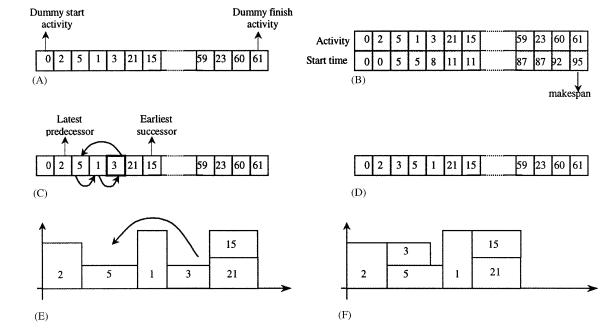
\includegraphics[scale=0.8]{sa.png}
  \caption{Representação de uma lista e processo de geração de um novo estado. (A) Representação de uma lista ordenada de tasks. (B) Exemplo de um planeamento viável com base na lista de tasks. (C) Geração aleatório de uma nova posição para a task 3. (D) Nova lista após o deslocamento. (E) Representação gráfica do Estado Inicial. (F) Representação gráfica do Novo Estado.}
  \label{Simulated Annealing}
\end{figure}

\section{Trabalho Realizado}
\justify\normalsize
 As fases abordadas até ao presente relatório foram as duas primeiras. A arquitetura explicitada pelo diagrama de classes uml já foi implementada e a obtenção de solução por algoritmos genéticos encontra-se numa fase avançada. De facto, o grupo encontra-se a afinar o algoritmo genético implementado através de testes por forma a maximizar a sua eficiência.

\section{Testes}
\justify\normalsize
Por forma a garantir a integridade do sistema e tendo em vista a obtenção da melhor solução possível pretende-se aplicar testes intensivos e promenorizados forçando situações complexas para visionar a resposta do programa. Espera-se criar projetos com 30, 60 e 120 tarefas e, sobre estes, será feita a análise comparativa para observar o comportamento do sistema em situações de diferente complexidade. Outras opções analisadas serão projetos com mais tarefas do que membros e vice-versa. Isto permite uma melhor apreensão da extensão da solução criada. Para além disto, o sistema será observado em situações de projetos com membros com listas de competências iguais ou diferentes. Finalmente, serão esmiuçadas situações com projetos apenas com tarefas sem precedências ou simplesmente tarefas com precedências.


\section{Conclusões}
\justify\normalsize
Em suma, verifica-se que o projeto se encontra a ser desenvolvido a um ritmo coeso e coerente, o que indica uma progressão saudável do mesmo. As fases encontram-se claramente delineadas o que permite uma maior eficácia na distribuição de tarefas entre os membros do grupo e, ao que tudo indica, levará à construção de um projeto bem documentado e estruturado.

O projeto escolhido despoletou a curiosidade de todos os membros. Apesar de por vezes serem encontradas dificuldades, são estas que dão alento ao estudo mais aprofundado das matérias abordadas e permitem um avanço sólido do mesmo. Espera-se que o trabalho a realizar no futuro se encontre dentro dos paradigmas do que já se encontra feito.

\bibliography{title_page_1}
\bibliographystyle{plain}

\end{titlepage}
\end{document}